At a high level, all of our models share the same two part structure: 
\textit{i) a sentence encoder} which maps an arbitrary sequence of tokens to 
an embedding $\sentvec \in \mathcal{R}^d$, and 
\textit{ii) a sentence extractor} which takes as input all of a document's 
sentence embeddings and predicts which sentences to extract to produce the 
extract summary. The sentence extractor is essentially a discriminative 
classifier $p(\slabel_1, \ldots, \slabel_{\docsize}| \sentvec_1, \ldots, \sentvec_{\docsize})$.

Depending on the architectural choices of each component we propose we 
can recover the specific implementations of \cite{cheng&lapata} and 
\cite{nallapati}, which we outline below.


\subsection{Sentence Encoders}
\begin{figure}
    \center
    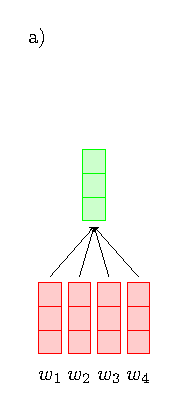
\includegraphics[scale=.75]{figures/avgsentencoder.pdf}
    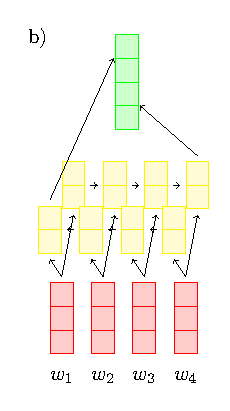
\includegraphics[scale=.75]{figures/rnnsentencoder.pdf}
    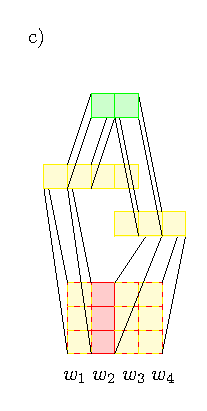
\includegraphics[scale=.75]{figures/cnnsentencoder.pdf}
    \caption{Sentence encoder architectures: a) averaging encoder, b) RNN encoder c) CNN encoder.}
    \label{fig:encoders}
\end{figure}



%TODO Perhaps add rnn with average pooling
We treat each sentence $\sent = \{\wemb_1, \ldots, \wemb_{|\sent|}\}$ 
as a sequence of word embeddings, where $|\sent|$ is the total number of words
in the sentence. We experiment with three architectures for mapping sequences
of word embeddings to a fixed length vector: average pooling, RNNs, and CNNs.

\textbf{Average Pooling} Average pooling is the simplest method and parameter
free. A sentence encoding $\operatorname{enc}(\sent) = 
\frac{1}{|\sent|} \sum_{\wemb \in \sent} \wemb$.

\textbf{RNN Encoder} Our second sentence encoder uses the concatenation of the
final output states of a forward and backward RNN over the sentence's word
embeddings. We use a Gated Recurrent Unit (GRU) \cite{cho} for the RNN cell,
since it has fewer parameters than the equivalent LSTM but with similar 
performance.

\begin{align} 
    \overrightarrow{h_i} &= \overrightarrow{\operatorname{GRU}}(w_i, h_{i-1}) \;\; \forall i \in 1, \ldots, |\sent| \\
    \overleftarrow{h_i} &= \overleftarrow{\operatorname{GRU}}(w_i, h_{i+1})  \;\; \forall i \in 1, \ldots, |\sent| \\
    \operatorname{enc}(s) &= [\overrightarrow{h_{|\sent|}} ; \overleftarrow{h_1} ] 
\end{align}

\textbf{CNN Encoder} Our final sentence encoder uses a series of 
convolutional feature maps to encode each sentence. This encoder is similar
to the convolutional architecture of \cite{kim} used for text classification
tasks and performs a series of ``one-dimensional'' convolutions over 
a sentence's associated word embeddings. 
In addition to its learned parameters, the CNN encoder has hyperparameters
associated to the window size of the convolutional filter 
(i.e. the number of words associated with each convolution) and the number of 
feature maps associated with each filter (i.e. the output dimension of each 
convolution). The CNN sentence encoding is computed as follows:

\begin{align}
 \specActivation_i &= \specConvBias 
    + \sum^\filterWindowSize_{j=1} \specConvWeight_j \cdot \wemb_{i + j -1}\\
  \specFeatureMap &= \max_{i\in 1,\dots, |\sent| - \filterWindowSize + 1} 
                      \relu\left(\specActivation_i\right) \\
                      \senc(s) &= \left[\specFeatureMap| \forall \numFeatureMaps \in \maxFeatureMaps, \filterWindowSize \in \maxWindowSize \right]
\end{align}


%\subsection{Sentence Extractors}
%\begin{figure*}
%    \center
%    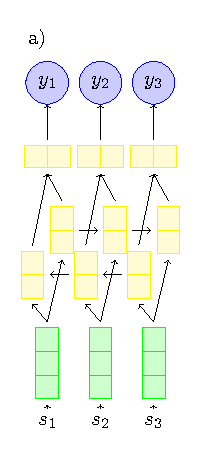
\includegraphics[scale=.75]{plots/rnnextractor.pdf}
%    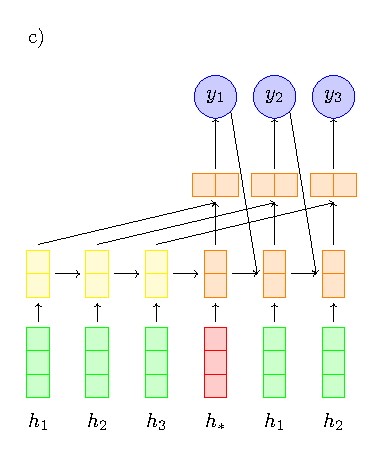
\includegraphics[scale=.75]{plots/clextractor.pdf}
%    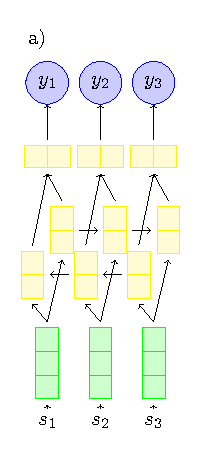
\includegraphics[scale=.75]{plots/rnnextractor.pdf}
%    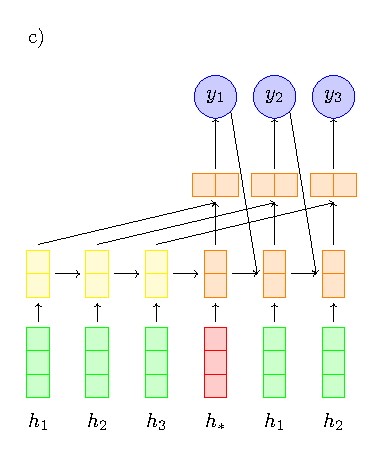
\includegraphics[scale=.75]{plots/clextractor.pdf}
%    \caption{This is a figure!}
%\end{figure*}
%
%
%Given a sequence of sentence embeddings $\sentvec_i = \senc(\sent_i)$,
%a sentence extractor produces a conditional distribution over the 
%corresponding sentence extraction variables 
%$p(\slabel_1,\ldots,\slabel_{\sentSize}|\sentvec_1, \ldots, \sentvec_{\sentSize})$.
%We propose two simple recurrent neural network based sentence extractors
%that make a strong conditional independence assumption over the labels
%$\slabel_i$,chiefly 
%$\explicitLikelihood= \naiveLikelihood$. This stands in contrast to our 
%baseline models which make a weaker assumption, 
%$\compactLikelihood = \markovLikelihood$, at the expense of greater 
%computational complexity. 
%
%\textbf{RNN Extractor} Our first proposed model is a very simple bidirectional
%RNN based tagging model. As in the RNN sentence encoder we use a GRU cell.
%The the forward and backward outputs of each sentence are passed through a 
%single layer perceptron with a sigmoid output to predict the probability
%of extracting each sentence:
%\begin{align}
%    \rExtHidden_i &= \rgru(\sentvec_i, \rExtHidden_{i-1}) \\
%   \lExtHidden_i &= \lgru(\sentvec_i, \lExtHidden_{i+1}) \\
%   \logits_i &= \relu\left(U \cdot [\rExtHidden_i; \lExtHidden_i] + u \right)\\
%   p(\slabel_i=1|\sentvec) &= \sigma\left(V\cdot \logits_i + v  \right).
%\end{align}
%
%\textbf{\sts~Extractor} One shortcoming of the RNN extractor is that long range
%information from one end of the document may not easily be able to effect 
%extraction probabilities of sentences at the other end. To mitigate this effect
%we introduce a \sts extractor based on the attentional seq2seq models commonly
%used for neural machine translation \cite{badhanau} and 
%abstractive summarization \cite{see}. The sentence embeddings are first
%encoded by a bidirectional $\gru$. A separate decoder $\gru$ transforms each 
%sentence into a query vector which attends to the encoder output. The
%attention weighted encoder output and the decoder $\gru$ output are concatenated
%and fed into a multi-layer percepron to compute the extraction probability.
%Formally we have:
%\begin{align}
%    \rEncExtHidden_i &= \rgru_{enc}(\sentvec_i, \rEncExtHidden_{i-1}) \\
%    \lEncExtHidden_i &= \lgru_{enc}(\sentvec_i, \lEncExtHidden_{i+1}) \\
%    \rDecExtHidden_i &= \rgru_{dec}(\sentvec_i, \rDecExtHidden_{i-1}) \\
%    \lDecExtHidden_i &= \lgru_{dec}(\sentvec_i, \lDecExtHidden_{i+1}) \\
%    \alpha_{i,j} &= \frac{\exp \left(\rDecExtHidden_j\cdot \rEncExtHidden_i + 
%\lDecExtHidden_j \cdot \lEncExtHidden_i \right)}{
%    \sum_{j=1}^{\docsize} \exp \left(\rDecExtHidden_j\cdot \rEncExtHidden_i + 
%\lDecExtHidden_j \cdot \lEncExtHidden_i \right) }\\
%\attnExtHidden_i &= \sum_{j=1}^{\docsize} 
%\alpha_{i,j} [\rEncExtHidden_j ;  \lEncExtHidden_j] \\
%   \logits_i &= \relu\left(U \cdot [\attnExtHidden_i; \rDecExtHidden_i; \lDecExtHidden_i] + u \right)\\
%   p(\slabel_i=1|\sentvec) &= \sigma\left(V\cdot \logits_i + v  \right).
%\end{align}
%
%\textbf{Cheng \& Lapata Extractor} 
%
%\begin{align}
%    \encExtHidden_i &= \gru_{enc}(\sentvec_i, \encExtHidden_{i-1}) \\
%    \decExtHidden_i &= \gru_{dec}(p_{i-1} \cdot \sentvec_{i-1}, \decExtHidden_{i-1}) \\
%   \logits_i &= \relu\left(U \cdot [\encExtHidden_i; \decExtHidden_i] + u \right)\\
%    p_i &= p(\slabel_i=1|\slabel_{<i}, \sentvec) = \sigma\left(V\cdot \logits_i + v  \right) 
%\end{align}
%
%
%\textbf{SummaRunner Extractor}
%\begin{align}
%    \rEncExtHidden_i &= \rgru(\sentvec_i, \rEncExtHidden_{i-1}) \\
%    \lEncExtHidden_i &= \lgru(\sentvec_i, \lEncExtHidden_{i+1}) \\
%    q &= \tanh\left(b_q + W_q\frac{1}{\docsize}\sum_{i=1}^{\docsize} [\rEncExtHidden_i; \lEncExtHidden_i] \right)\\
%    \extHidden_i &= \relu\left(b_z + W_z [\rEncExtHidden_i; \lEncExtHidden_i]\right)
%  \end{align}
%  \begin{align*}
%      p(y_i=1|y_{<i}, h) = \sigma(& W_{con}\cdot z_i \\
%                     & + z_i^T W_{sal}\cdot q \\
%                     & -z_i^T W_{nov} \cdot \tanh(g_i) \\
%                     & + b_{rp_i}  \\
%                     & + b_{ap_i} \\
%                     & + b)     \\
%      g_j & = \sum_{i=1}^{j-1} p(y_j=1|y_{<j},h) \cdot z_j
%\end{align*}


